\begin{markdown}

\clearpage
# Reverse Engineering Exercise 2: Crack me

**[Binary Provided: `2010303027_hw_1_exercise_2.exe`]**

## Fingerprint the program using any of the hashing tools that were presented during the lecture.

Here's a small report from HashMyfiles:\s

* Filename: `2010303027_hw_1_exercise_2.exe`
* MD5: `456809322ef371ca13c40b2626baa6a5`
* SHA1: `57fb1a64eb6099da090b063bd3e0e140f66cfa05`
* CRC32: `f6093492`

\noindent\s SHA-256: **`fc3a851c9958f5cafc9b04ffa4afae346c4633355e0d2d6f8a6b0f2292cef58e`**

## Run the program and enter an input value.

* What input value did you use? 

\noindent\s `123`

* What did you receive as an output?

\end{markdown}
\begin{lstlisting}[name={output pattern for input `123`}]
****
****
***:
*#*@
\end{lstlisting}
\begin{markdown}

---

\noindent\s I've continued to try values until I found the following pattern:

* `0`: `**`
* `1`: `*:`
* `2`: `*#`
* `3`: `*@`
* `4`: `:*`
* `5`: `::`
* etc. until `Fh` which is `@@`

\noindent\s These can be represented as Nibbles.

---

\noindent\s Assumption: break it down further:
`0` is `0b0000` so one `0b00` could represents a single `*`
If we compare it with `1` which is `0b0001` this could mean `:` is `0b0001`. Let's create a mapping and compare it with the values we know from our previous experiment.\s

* `00`: `*`
* `01`: `:`
* `10`: `#`
* `11`: `@`

\noindent\s This mapping checks out.

## What’s the address of the program’s entry point?

**`403000h`**

---

This is set in the PE header. In IDA you can load it by:\s

* loading the binary with the `Manual load` option
* answering yes to `Load the file header?` dialogue

\noindent\s Now you can jump to the header (*g* `HEADER:0`) and look for the address of the entry point.

\begin{figure}[!htbp]
\centering
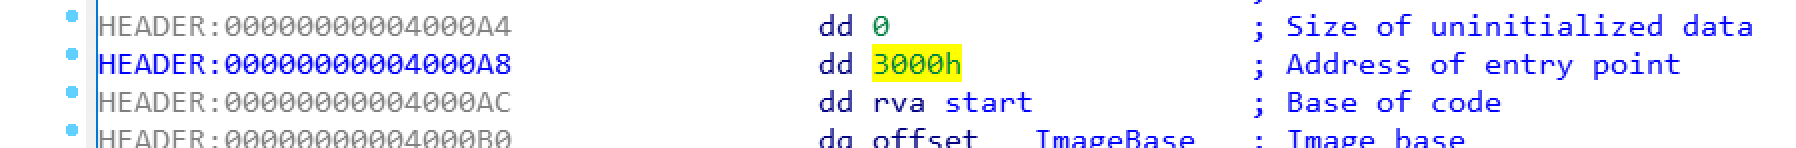
\includegraphics[width=\linewidth]{media/entry.png}
\caption{header of the }\label{entry}
\end{figure}

\noindent Adding this to the `image base` results in an address that is indeed the `start` of our program, see Figure \ref{entrypoint}.

\begin{figure}[!htbp]
\centering
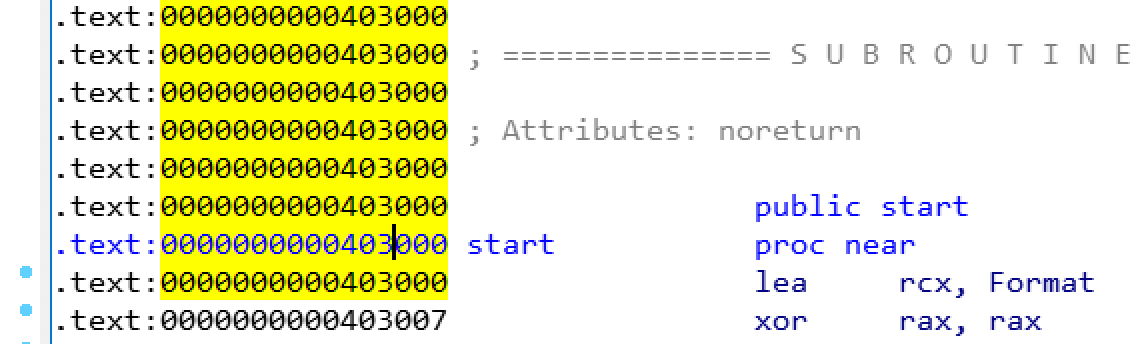
\includegraphics[width=\linewidth]{media/entrypoint.png}
\caption{the entry point of the second program}\label{entrypoint}
\end{figure}

\clearpage
## Identify the strings present in this program.

* Use one of the tools installed in the virtual analysis environment.

\noindent\s I'm really taking a shine to IDA so let's stick with that. There is a strings sub view, see Figure \ref{strings}.

\begin{figure}[!htbp]
\centering
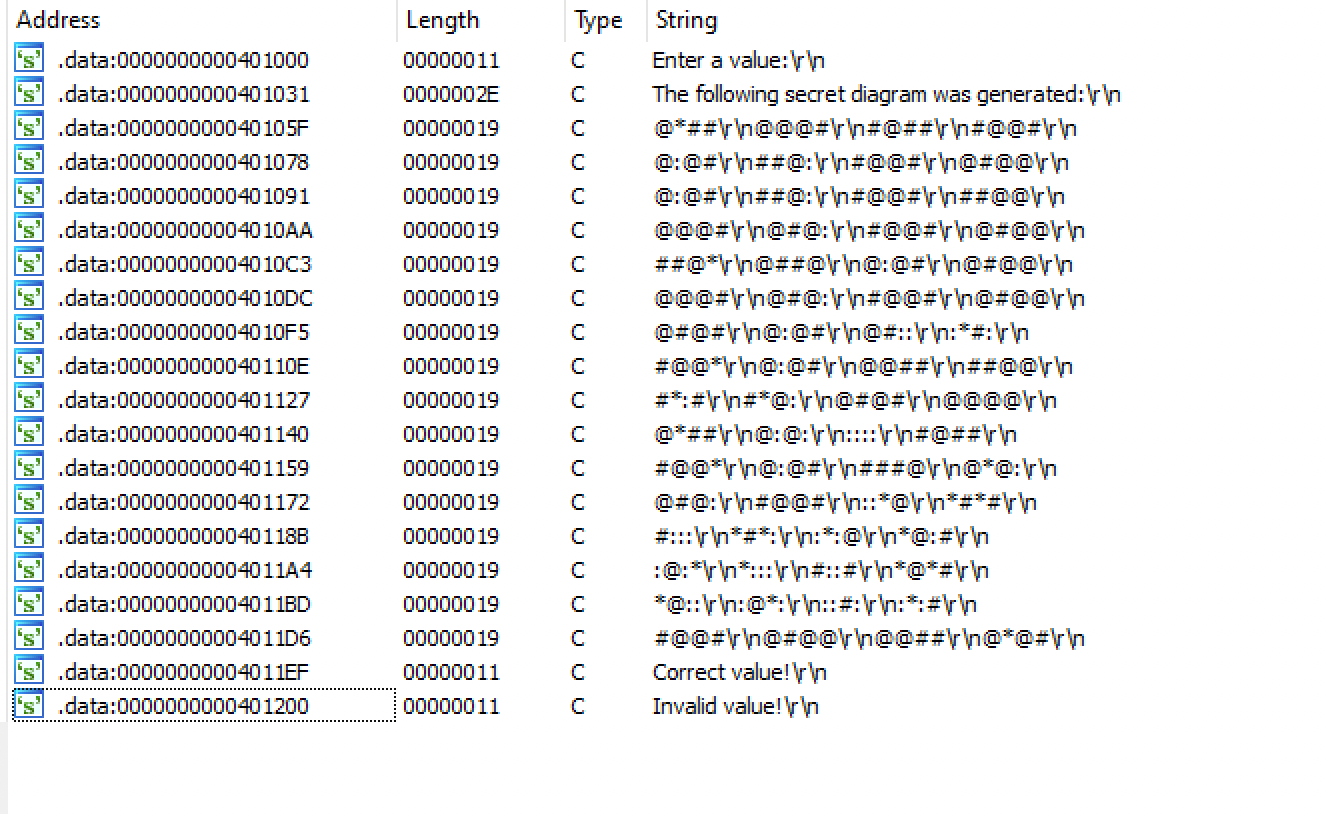
\includegraphics[width=\linewidth]{media/strings.png}
\caption{string sub view in IDA}\label{strings}
\end{figure}

There are a couple missing (like the DOS warning). Let's try it with `BinText`:\s

* load the binary
* include linefeed and carriage return in the `Filter` tab
    * to include strings from the secret diagram
* press `GO`

\end{markdown}
\begin{lstlisting}[name={more strings}]
00000000004D   0000C000008D      0   !This program cannot be run in DOS mode.
000000000188   000000000127      0   .data
0000000001D8   000000000177      0   .text
000000000200   00000000019F      0   .idata
# [...]
\end{lstlisting}
\begin{markdown}

Indeed a couple more that IDA hid from us!
## What sections are present in this program, what are their names and where are they located when the application is loaded into memory?

* Provide an address for each section

\noindent\s IDA provides a sub view for sections as well: see Figure \ref{sections}.\s

\begin{figure}[!htbp]
\centering
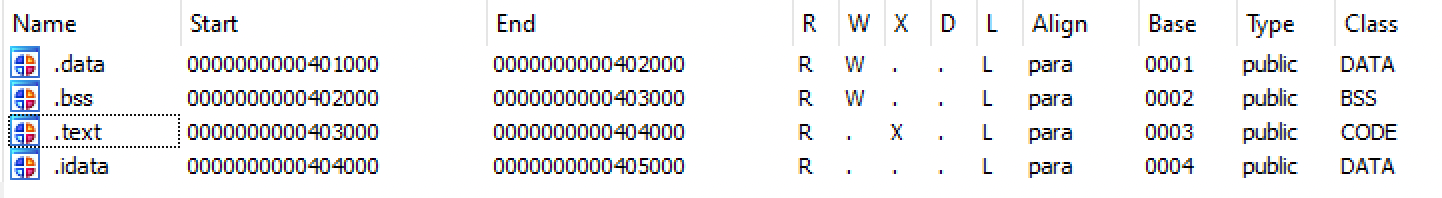
\includegraphics[width=\linewidth]{media/sections.png}
\caption{sections sub view in IDA}\label{sections}
\end{figure}

\noindent\s For the sake of readability, here are the section names and their respective start addresses:\s

* `.data`: `401000h`
* `.bss`: `402000h`
* `.text`: `403000h`
* `.idata`: `404000h`

## Identify all symbols that are imported by the program and their import directory (library)!

* Make sure you list all libraries that are linked to each import symbol and the address of each symbol
* Use a tool in the virtual analysis environment to make the search easier

\begin{figure}[!htbp]
\centering
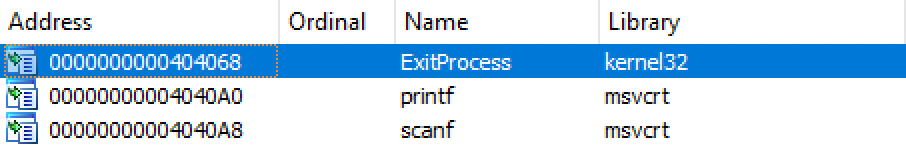
\includegraphics[width=\linewidth]{media/symbols.png}
\caption{imports sub view in IDA}\label{symbols}
\end{figure}

\clearpage
## Identify all exported symbols and their addresses

\begin{figure}[!htbp]
\centering
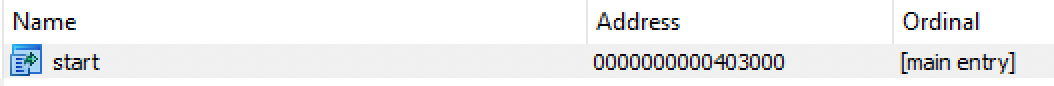
\includegraphics[width=\linewidth]{media/exports.png}
\caption{exports sub view in IDA}\label{export}
\end{figure}

## What calling convention is used by the following functions:

* `printf`
    * **x64 calling convention**
        * first parameter via `rcx`
        * similar to `__fastcall` but up to 4 instead of 2 registers
            * `rcx`, `rdx`, `r8`, `r9`
            * after that via the stack
* `scanf`
    * **x64 calling convention**
        * two parameters: `rcx` and `rdx`
* `sub_4030C7` (location `0x4030C7`)
    * **`__cdecl`**
        * cleaned up by caller (`add rsp, 10h`)
* `sub_403139` (location `0x403139`)
    * **`__stdcall`**
        * pushed to the stack: `401127h` and `402000h`
        * cleaned up by callee (`retn 10h`)
        
\begin{figure}[!htbp]
\centering
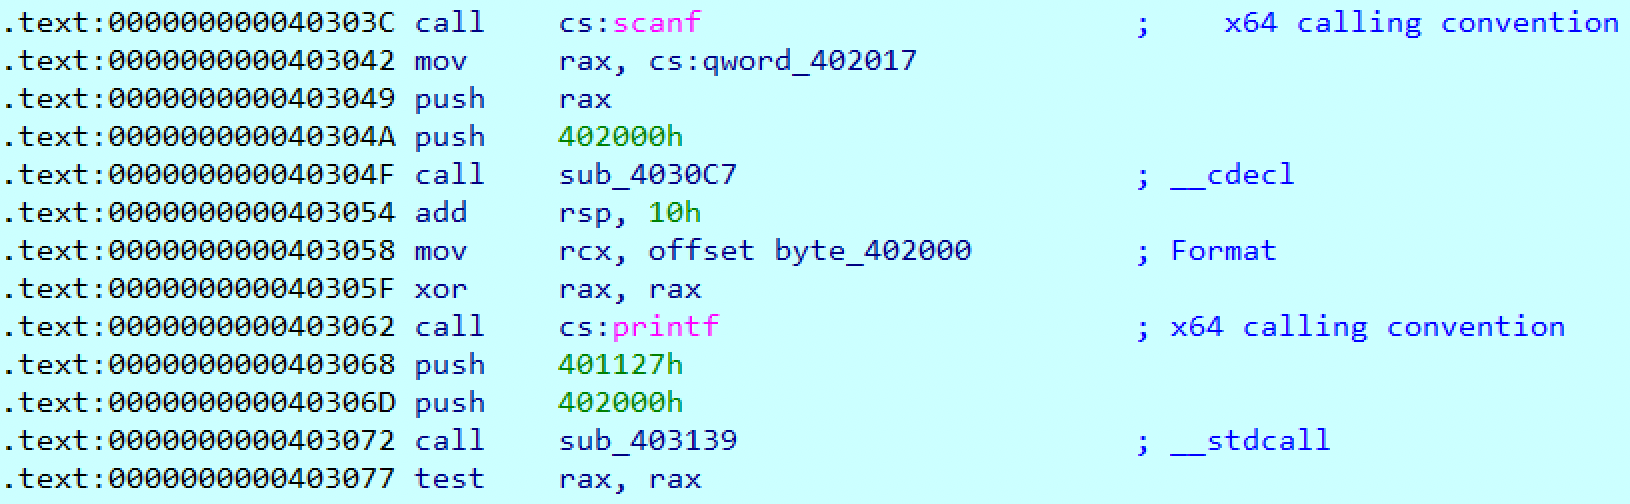
\includegraphics[width=\linewidth]{media/call.png}
\caption{calling conventions}\label{export}
\end{figure}

\noindent\s I've used Compile Explorer to play around with the different calling conventions with both x64 and x86 version of the `msvc` compiler: \href{https://godbolt.org/z/TcsToh}{https://godbolt.org/z/TcsToh}.

## Explain in your own words. What does this function do?

* `sub_4030A7` (location `0x4030A7`)

\noindent\s This function takes two bytes as input (via `rbx`) and returns a mapped character as an output (via `rax`).
\n
Possible input/output mappings:\s

* `00` -> `*`
* `01` -> `:`
* `10` -> `#`
* `11` -> `@`

---

\noindent Detailed order of operations (see figure \ref{a7}):
\n
\noindent This function is called in `sub_4030C7` via `.text:004030F5 call    sub_4030A7`. Before the call the following happens:\s

* `rbx` is nulled out everywhere but the 2 least significant bits (`and rbx, 3`)
* `rbx` is pushed to the stack as parameter for the call

\noindent\s If we assume that the user input is `ABCD1234`, the two least significant bits of `Ah` (`0b1010`) are `0b10`. This is the argument for the first time the function is called.
\n
In the function the following happens:\s

* `rbx` is pushed to the stack and popped to the lower `ebx`
* `rax` is set to `@` (`40h`, as a default value)
* the lowest byte of `ebx` is written written back, the upper filled with zeros
* `ebx` is compared with `0b11`:
    * if `ebx` is not bigger than `3`: use it as array lookup index and write value to `rax`
    * else: jump past array lookup (keeping the default value for `rax`)
* restore `ebp`
* exit

\noindent\s After the function the rest of the program can work with the return value (stored in `rax`).

\begin{figure}[!htbp]
\centering
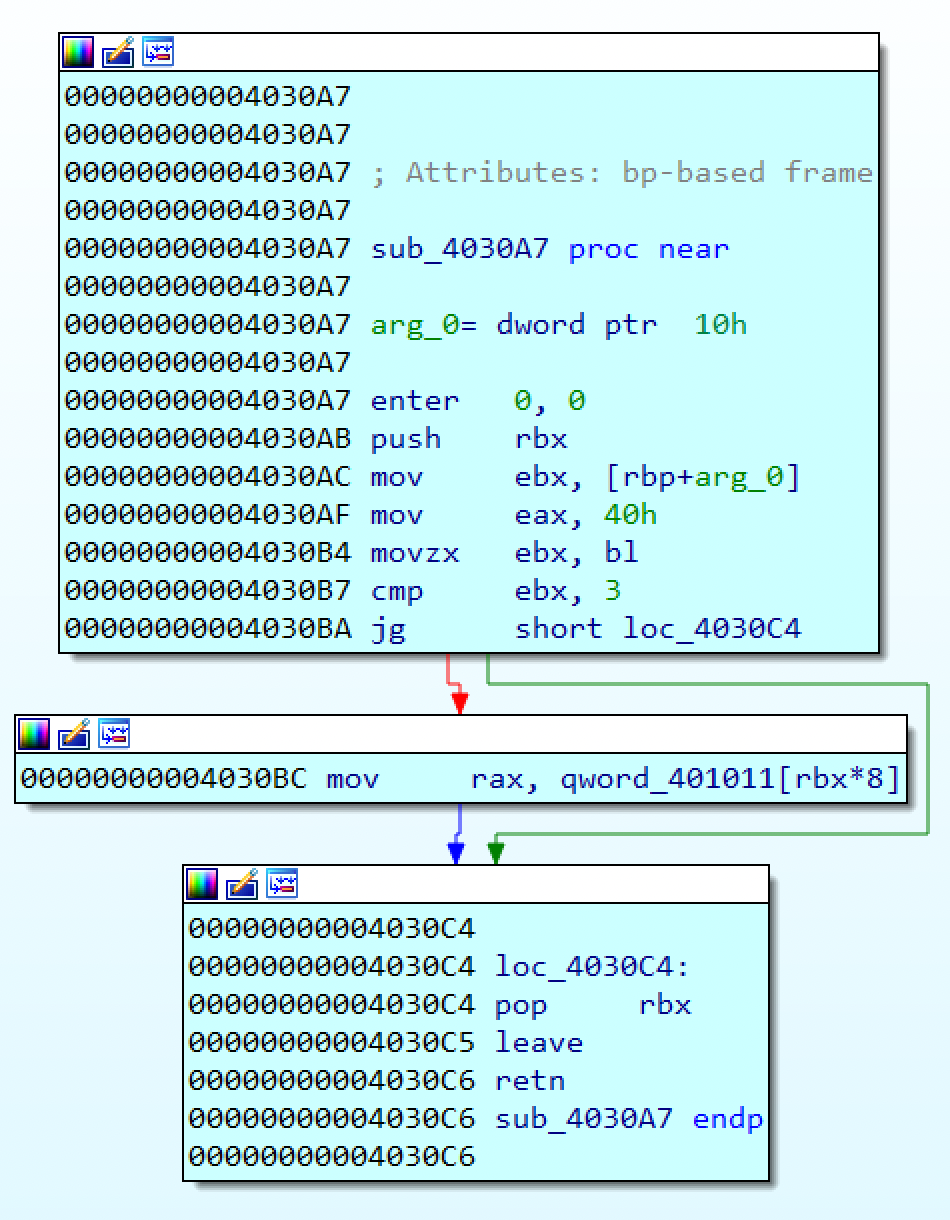
\includegraphics[width=0.8\linewidth]{media/a7.png}
\caption{the function `sub_4030A7`}\label{a7}
\end{figure}

## Figure out what code needs to be entered as an input in the console to match the diagram that is displayed. How did you find out?

* After the correct input has been provided, the following message should appear “Correct value!”

\noindent\s The pattern:

\end{markdown}
\begin{lstlisting}[name={target secret pattern}]
#*:#
#*@:
@#@#
@@@@
\end{lstlisting}
\begin{markdown}

Using the mapping from task 2.2 (plus the confirmation from task 2.9) and a bit of help from `calc.exe` we get: `868DEEFFh`. See Figure \ref{pattern} and Figure \ref{solution}.

\begin{figure}[!htbp]
\centering
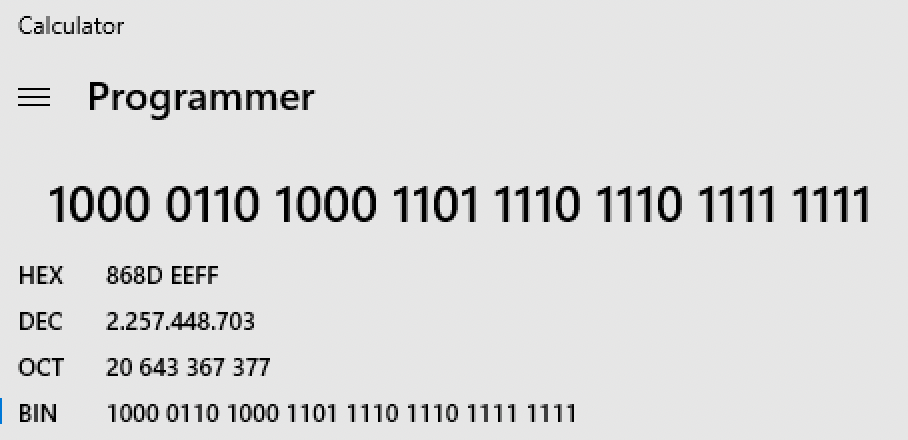
\includegraphics[width=\linewidth]{media/pattern.png}
\caption{converting the key from binary to hex}\label{pattern}
\end{figure}

\begin{figure}[!htbp]
\centering
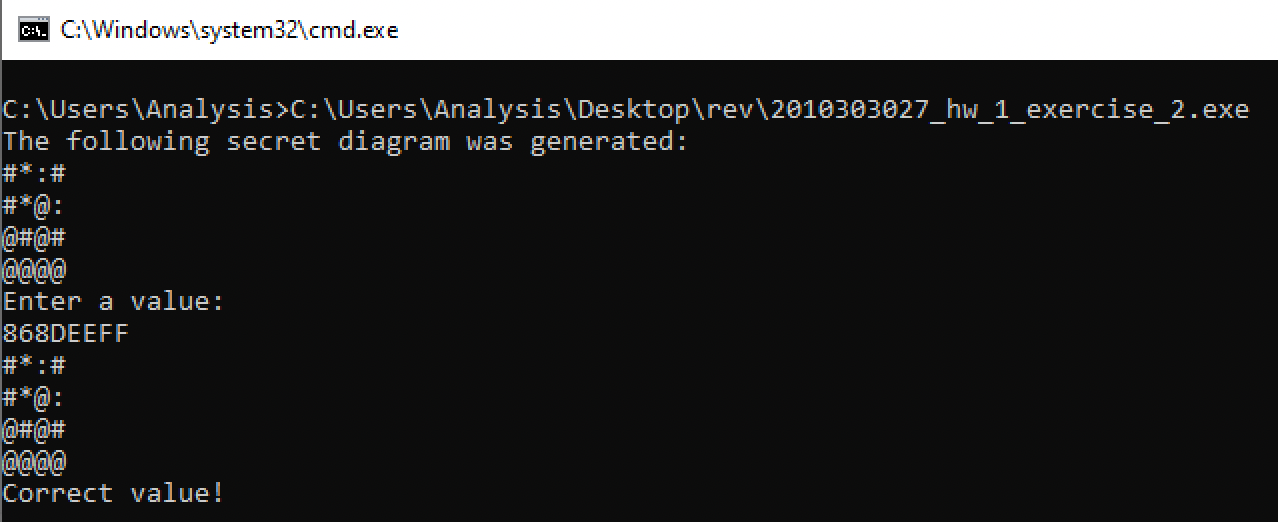
\includegraphics[width=1.1\linewidth]{media/solution.png}
\caption{checking the secret key}\label{solution}
\end{figure}

\end{markdown}